% Figure 6: TRL Progression Diagram
% Author: Dr. Computernonymouse
% Description: Technology Readiness Level timeline showing progression from
%              basic research to commercial deployment for ZPE technologies

\documentclass[tikz,border=10pt]{standalone}
\usepackage{tikz}
\usepackage{pgfplots}
\usepackage{amsmath}
\usepackage{amssymb}

\pgfplotsset{compat=1.18}
\usetikzlibrary{calc,arrows.meta,patterns,backgrounds,positioning,shapes.geometric,decorations.markings}

% Define TRL colors
\definecolor{achieved}{RGB}{70,191,70}
\definecolor{partial}{RGB}{255,192,0}
\definecolor{planned}{RGB}{255,99,71}
\definecolor{projected}{RGB}{176,196,222}
\definecolor{timeline}{RGB}{70,70,70}
\definecolor{milestone}{RGB}{0,0,139}

% TRL level descriptions
\def\trlOne{Basic principles observed}
\def\trlTwo{Technology concept formulated}
\def\trlThree{Proof of concept}
\def\trlFour{Component validation}
\def\trlFive{Component validation in relevant environment}
\def\trlSix{System prototype demonstration}
\def\trlSeven{System prototype in operational environment}
\def\trlEight{System complete and qualified}
\def\trlNine{System proven in operational environment}

\begin{document}

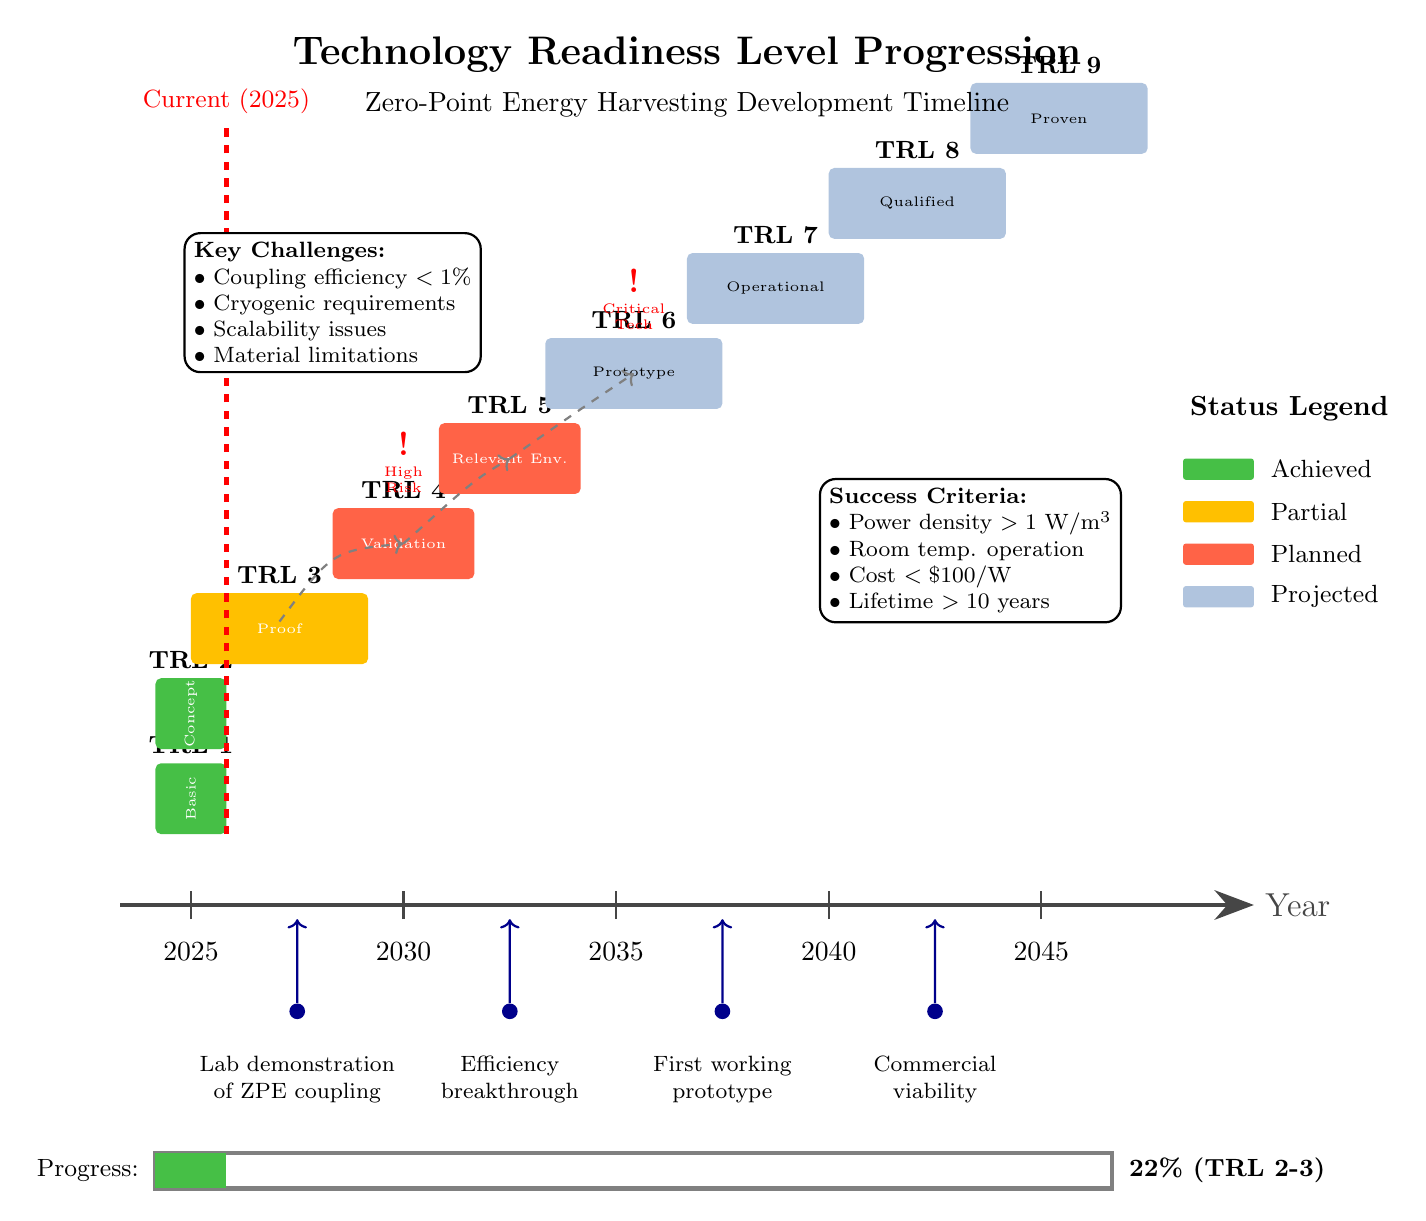
\begin{tikzpicture}[scale=0.9]

% Timeline axis
\draw[timeline,ultra thick,-{Stealth[length=5mm]}] (0,0) -- (16,0) node[right,font=\large] {Year};

% Year markers
\foreach \year/\x in {2025/1, 2030/4, 2035/7, 2040/10, 2045/13} {
    \draw[timeline,thick] (\x,-0.2) -- (\x,0.2);
    \node[below,font=\normalsize] at (\x,-0.4) {\year};
}

% TRL level bars
\begin{scope}[yshift=1cm]
    % TRL 1 - Achieved (Green)
    \fill[achieved,rounded corners=2pt] (0.5,0) rectangle (1.5,1);
    \node[above,font=\small\bfseries] at (1,1) {TRL 1};
    \node[rotate=90,font=\tiny,white] at (1,0.5) {Basic};

    % TRL 2 - Achieved (Green)
    \fill[achieved,rounded corners=2pt] (0.5,1.2) rectangle (1.5,2.2);
    \node[above,font=\small\bfseries] at (1,2.2) {TRL 2};
    \node[rotate=90,font=\tiny,white] at (1,1.7) {Concept};

    % TRL 3 - Partial (Yellow) - Current status
    \fill[partial,rounded corners=2pt] (1,2.4) rectangle (3.5,3.4);
    \node[above,font=\small\bfseries] at (2.25,3.4) {TRL 3};
    \node[font=\tiny,white] at (2.25,2.9) {Proof};
    \draw[ultra thick,red,dashed] (1.5,0) -- (1.5,10) node[above,font=\small] {Current (2025)};

    % TRL 4 - Planned (Red)
    \fill[planned,rounded corners=2pt] (3,3.6) rectangle (5,4.6);
    \node[above,font=\small\bfseries] at (4,4.6) {TRL 4};
    \node[font=\tiny,white] at (4,4.1) {Validation};

    % TRL 5 - Planned (Red)
    \fill[planned,rounded corners=2pt] (4.5,4.8) rectangle (6.5,5.8);
    \node[above,font=\small\bfseries] at (5.5,5.8) {TRL 5};
    \node[font=\tiny,white] at (5.5,5.3) {Relevant Env.};

    % TRL 6 - Projected (Light Blue)
    \fill[projected,rounded corners=2pt] (6,6) rectangle (8.5,7);
    \node[above,font=\small\bfseries] at (7.25,7) {TRL 6};
    \node[font=\tiny] at (7.25,6.5) {Prototype};

    % TRL 7 - Projected (Light Blue)
    \fill[projected,rounded corners=2pt] (8,7.2) rectangle (10.5,8.2);
    \node[above,font=\small\bfseries] at (9.25,8.2) {TRL 7};
    \node[font=\tiny] at (9.25,7.7) {Operational};

    % TRL 8 - Projected (Light Blue)
    \fill[projected,rounded corners=2pt] (10,8.4) rectangle (12.5,9.4);
    \node[above,font=\small\bfseries] at (11.25,9.4) {TRL 8};
    \node[font=\tiny] at (11.25,8.9) {Qualified};

    % TRL 9 - Projected (Light Blue)
    \fill[projected,rounded corners=2pt] (12,9.6) rectangle (14.5,10.6);
    \node[above,font=\small\bfseries] at (13.25,10.6) {TRL 9};
    \node[font=\tiny] at (13.25,10.1) {Proven};
\end{scope}

% Key milestones
\node[milestone,circle,fill=milestone,inner sep=2pt] (m1) at (2.5,-1.5) {};
\draw[milestone,thick,->] (m1) -- (2.5,-0.2);
\node[below,align=center,font=\footnotesize] at (2.5,-2) {
    Lab demonstration\\of ZPE coupling
};

\node[milestone,circle,fill=milestone,inner sep=2pt] (m2) at (5.5,-1.5) {};
\draw[milestone,thick,->] (m2) -- (5.5,-0.2);
\node[below,align=center,font=\footnotesize] at (5.5,-2) {
    Efficiency\\breakthrough
};

\node[milestone,circle,fill=milestone,inner sep=2pt] (m3) at (8.5,-1.5) {};
\draw[milestone,thick,->] (m3) -- (8.5,-0.2);
\node[below,align=center,font=\footnotesize] at (8.5,-2) {
    First working\\prototype
};

\node[milestone,circle,fill=milestone,inner sep=2pt] (m4) at (11.5,-1.5) {};
\draw[milestone,thick,->] (m4) -- (11.5,-0.2);
\node[below,align=center,font=\footnotesize] at (11.5,-2) {
    Commercial\\viability
};

% Legend
\begin{scope}[shift={(16.5,3)}]
    \node[font=\normalsize\bfseries,align=center] at (0,4) {Status Legend};

    \fill[achieved,rounded corners=1pt] (-1.5,3) rectangle (-0.5,3.3);
    \node[right,font=\small] at (-0.4,3.15) {Achieved};

    \fill[partial,rounded corners=1pt] (-1.5,2.4) rectangle (-0.5,2.7);
    \node[right,font=\small] at (-0.4,2.55) {Partial};

    \fill[planned,rounded corners=1pt] (-1.5,1.8) rectangle (-0.5,2.1);
    \node[right,font=\small] at (-0.4,1.95) {Planned};

    \fill[projected,rounded corners=1pt] (-1.5,1.2) rectangle (-0.5,1.5);
    \node[right,font=\small] at (-0.4,1.35) {Projected};
\end{scope}

% Critical path dependencies
\draw[thick,gray,dashed,->] (2.25,4) .. controls (3,5) .. (4,5.1);
\draw[thick,gray,dashed,->] (4,5.1) .. controls (5,6) .. (5.5,6.3);
\draw[thick,gray,dashed,->] (5.5,6.3) .. controls (6.5,7) .. (7.25,7.5);

% Risk indicators
\node[red,font=\large\bfseries] at (4,6.5) {!};
\node[red,align=center,font=\tiny] at (4,6) {High\\Risk};

\node[red,font=\large\bfseries] at (7.25,8.8) {!};
\node[red,align=center,font=\tiny] at (7.25,8.3) {Critical\\Tech};

% Title and subtitle
\node[font=\Large\bfseries] at (8,12) {Technology Readiness Level Progression};
\node[font=\normalsize] at (8,11.3) {Zero-Point Energy Harvesting Development Timeline};

% Key challenges box
\node[draw=black,thick,rounded corners=2mm,fill=white!90,
      align=left,font=\footnotesize] at (3,8.5) {
    \textbf{Key Challenges:}\\
    $\bullet$ Coupling efficiency $< 1\%$\\
    $\bullet$ Cryogenic requirements\\
    $\bullet$ Scalability issues\\
    $\bullet$ Material limitations
};

% Success criteria box
\node[draw=black,thick,rounded corners=2mm,fill=white!90,
      align=left,font=\footnotesize] at (12,5) {
    \textbf{Success Criteria:}\\
    $\bullet$ Power density $> 1$ W/m$^3$\\
    $\bullet$ Room temp. operation\\
    $\bullet$ Cost $< \$100$/W\\
    $\bullet$ Lifetime $> 10$ years
};

% Progress indicator
\draw[ultra thick,gray] (0.5,-3.5) rectangle (14,-4);
\fill[achieved] (0.5,-3.5) rectangle (1.5,-4);
\node[left,font=\small] at (0.4,-3.75) {Progress:};
\node[right,font=\small\bfseries] at (14.1,-3.75) {22\% (TRL 2-3)};

\end{tikzpicture}

\end{document}